\documentclass[12pt,a4paper]{article}

\usepackage[utf8]{inputenc}
\usepackage[T1]{fontenc}
\usepackage{amsmath, amssymb, amsthm, mathtools}
\usepackage{physics}
\usepackage{geometry}
\usepackage{graphicx}
\usepackage{hyperref}
\usepackage{caption}
\usepackage{float}
\usepackage{bm}
\usepackage{cite}
\geometry{margin=1in}

\title{Advanced Mathematical Modeling of Antimatter Dynamics in Strong Gravitational Fields}
\author{Mari Harbi}
\date{\today}

\begin{document}

\maketitle

\begin{abstract}
This paper presents a comprehensive mathematical framework to study the dynamics of antimatter in strong gravitational fields. Starting from relativistic field equations (Dirac and Klein--Gordon) in curved spacetime, we derive the Hamiltonian formulation suitable for time evolution. Analytical and numerical methods (perturbation expansion, spectral decomposition) are developed to compute bound states and correlation functions. Observables such as probability densities, currents, and Wigner functions are extracted to visualize the quantum state distribution in phase space. Each equation is motivated and linked to the final goal: modeling antimatter under strong gravity.
\end{abstract}

\section{Motivation}
Studying antimatter in strong gravity is essential to:  
1. Understand whether antimatter can exist near high-density regions such as neutron stars or black holes.  
2. Explore the role of gravitational effects on matter-antimatter asymmetry in the universe.  

The practical goal is to build a coherent set of equations that lead from fundamental field equations to measurable predictions (local probability densities, annihilation rates, local energy spectra).

\section{Geometrical Framework — Metric, Tetrad, and Spin Connection}
We define the geometric tools required to write spinor equations in curved spacetime.

\subsection{Metric and Vierbein}
The general metric:
\[
g_{\mu\nu}(x)
\]
and the vierbein \(e_\mu^{\;a}(x)\):
\[
g_{\mu\nu}(x)=e_\mu^{\;a}(x)\,e_\nu^{\;b}(x)\,\eta_{ab},\qquad \eta_{ab}=\mathrm{diag}(-1,1,1,1)
\]
with inverse \(e^\mu_{\;a}\) such that \(e^\mu_{\;a} e_\mu^{\;b}=\delta_a^b\).

\paragraph{Practical explanation:} The vierbein connects curved spacetime indices (Greek) to local flat indices (Latin), allowing local gamma matrices \(\gamma^a\) to be mapped as \(\gamma^\mu(x)=e^\mu_{\;a}(x)\gamma^a\).

\subsection{Christoffel Symbols and Spin Connection}
\[
\Gamma^\lambda_{\mu\nu}=\tfrac{1}{2} g^{\lambda\sigma}(\partial_\mu g_{\nu\sigma}+\partial_\nu g_{\mu\sigma}-\partial_\sigma g_{\mu\nu})
\]
Spin connection:
\[
\omega_{\mu}^{\;ab}=e^{a}_{\;\nu}(\partial_\mu e^{\nu b}+\Gamma^\nu_{\mu\sigma} e^{\sigma b}),\quad
\Gamma_\mu=\tfrac{1}{4}\,\omega_{\mu}^{\;ab}\,\gamma_a\gamma_b
\]
ensuring the tetrad is covariantly constant: \(\nabla_\mu e_\nu^{\;a}=0\).

\section{Field Equations in Curved Spacetime}
\subsection{Dirac Equation}
Covariant derivative:
\[
\nabla_\mu\psi=\partial_\mu\psi+\Gamma_\mu\psi
\]
Dirac equation:
\begin{equation}\label{eq:dirac_cov}
(i\gamma^\mu(x)\nabla_\mu - m)\psi(x)=0
\end{equation}

\paragraph{Explanation:}  
- \(\gamma^\mu(x)=e^\mu_{\;a}\gamma^a\) depends on position.  
- \(\Gamma_\mu\) incorporates spin rotation due to curvature.  
- This ensures local Lorentz invariance and general covariance.

Expanded form:
\[
i\gamma^\mu\partial_\mu\psi + i\gamma^\mu\Gamma_\mu\psi - m\psi = 0
\]

\subsection{Klein--Gordon Equation}
For a scalar field:
\begin{equation}\label{eq:kg_curved}
(\Box + m^2 + \xi R)\phi(x) = 0, \quad
\Box=\frac{1}{\sqrt{-g}}\partial_\mu(\sqrt{-g}g^{\mu\nu}\partial_\nu)
\end{equation}
\paragraph{Explanation:}  
- \(\xi R\) is the curvature coupling; \(\xi=0\) is minimal, \(\xi=1/6\) is conformal.  
- \(\Box\) reflects the curved spacetime D'Alembertian.

\section{Hamiltonian Formulation}
Assuming a stationary metric (\(\partial_t\) Killing vector), we write:
\[
i\hbar \partial_t\psi = H_{\mathrm{Dirac}}\psi
\]
with
\begin{equation}\label{eq:dirac_ham}
H_{\mathrm{Dirac}} = -i\hbar \alpha^i(x)(\nabla_i+\Gamma_i) + \beta m + V_{\mathrm{grav}}(x)
\end{equation}
\paragraph{Explanation:}  
- \(\alpha^i(x)=\gamma^0\gamma^i(x)\), \(\beta=\gamma^0\)  
- \(V_{\mathrm{grav}}(x)\) is the gravitational potential contribution.  

KG equation as eigenvalue problem:
\[
(-\Delta_{\mathrm{curved}} + V_{\mathrm{eff}}(\mathbf{x}))\chi(\mathbf{x}) = \omega^2 \chi(\mathbf{x})
\]

\section{Perturbation Theory}
Weak-field approximation:
\[
g_{\mu\nu}=\eta_{\mu\nu}+h_{\mu\nu},\quad |h_{\mu\nu}|\ll 1
\]
Hamiltonian:
\[
H=H_0 + \lambda V,\quad \lambda\sim O(h)
\]

Perturbative expansion:
\[
\psi(t)=\psi^{(0)}(t)+\lambda\psi^{(1)}(t)+\lambda^2\psi^{(2)}(t)+\dots
\]
First-order correction:
\[
i\hbar\partial_t\psi^{(1)} = H_0\psi^{(1)} + V\psi^{(0)},\quad
\psi^{(1)}(t) = -\frac{i}{\hbar}\int_{t_0}^t U_0(t,t')\,V\,\psi^{(0)}(t')\,dt'
\]

\section{Spectral Methods}
Basis choice:
\[
\phi_{n\ell m}(r,\theta,\phi)=R_{n\ell}(r)\,Y_\ell^m(\theta,\phi)
\]
Hamiltonian matrix:
\[
H_{n\ell m; n'\ell' m'} = \int d^3x\,\phi_{n\ell m}^\dagger(\mathbf{x})\,H(\mathbf{x})\,\phi_{n'\ell' m'}(\mathbf{x})
\]
Time evolution:
\[
i\hbar \dot{\mathbf{c}}(t) = \mathbf{H}\mathbf{c}(t)
\]

\section{Observables}
Probability density and current:
\[
\rho(x,t)=\psi^\dagger\psi,\quad j^\mu = \bar\psi \gamma^\mu \psi, \quad \nabla_\mu j^\mu = 0
\]
Wigner function:
\[
W(x,p,t)=\frac{1}{\pi\hbar}\int dy\, e^{2 i p y/\hbar}\,\psi^*(x+y,t)\psi(x-y,t)
\]
Annihilation rate:
\[
\Gamma_{\rm ann} \sim \langle\sigma v\rangle \int d^3x\,\rho_{\rm matter}\rho_{\rm antimatter}
\]

\section{Bound States}
Bound state condition:
\[
\int d^3x\,|\chi(\mathbf{x})|^2 < \infty,\quad \omega^2 < V_\infty
\]

\section{Numerical Implementation}
Steps:
\begin{enumerate}
\item Choose metric (Schwarzschild/Kerr/neutron star).  
\item Compute vierbein and spin connection.  
\item Construct \(H_{\rm Dirac}\).  
\item Choose basis and compute \(H_{nm}\).  
\item Solve \(i\hbar \dot c = Hc\) numerically.  
\item Extract \(\rho, j^\mu, W, \Gamma_{\rm ann}\).  
\item Check bound states and parameter dependence.
\end{enumerate}

\section{Illustrative Figures}
\begin{figure}[H]
\centering
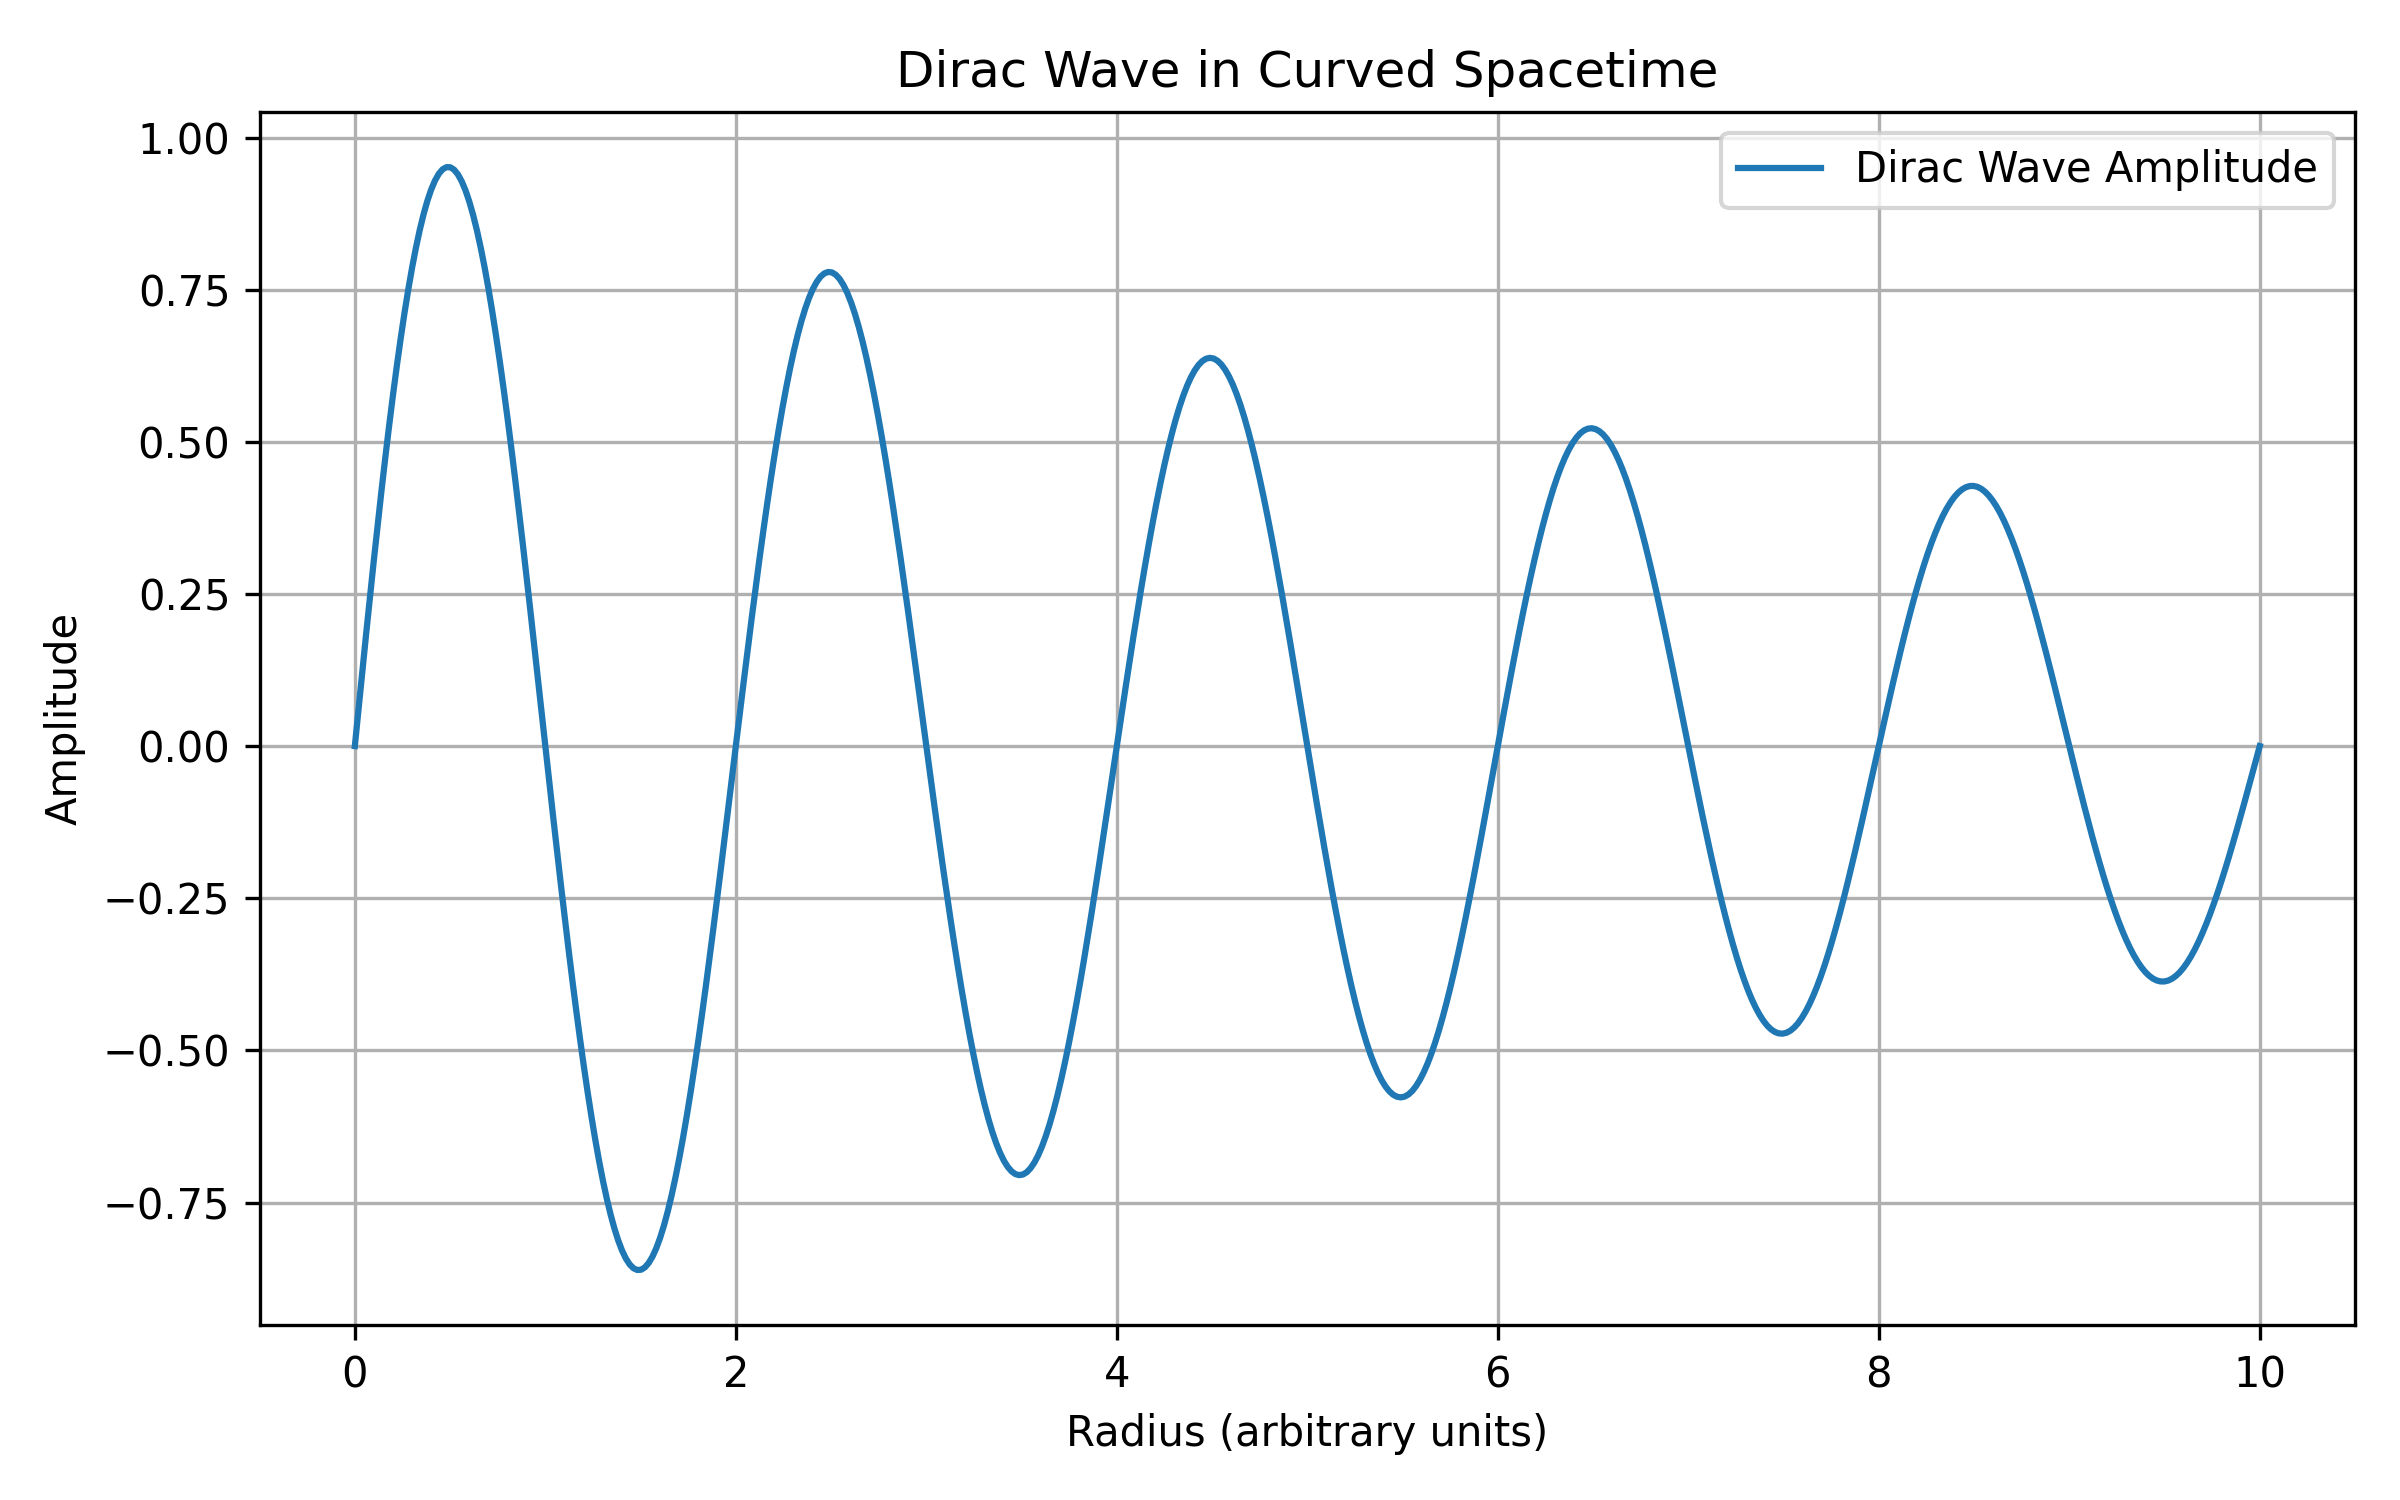
\includegraphics[width=0.8\textwidth]{dirac_curved.png}
\caption{Dirac wave behavior in curved spacetime (placeholder).}
\label{fig:dirac}
\end{figure}

\begin{figure}[H]
\centering
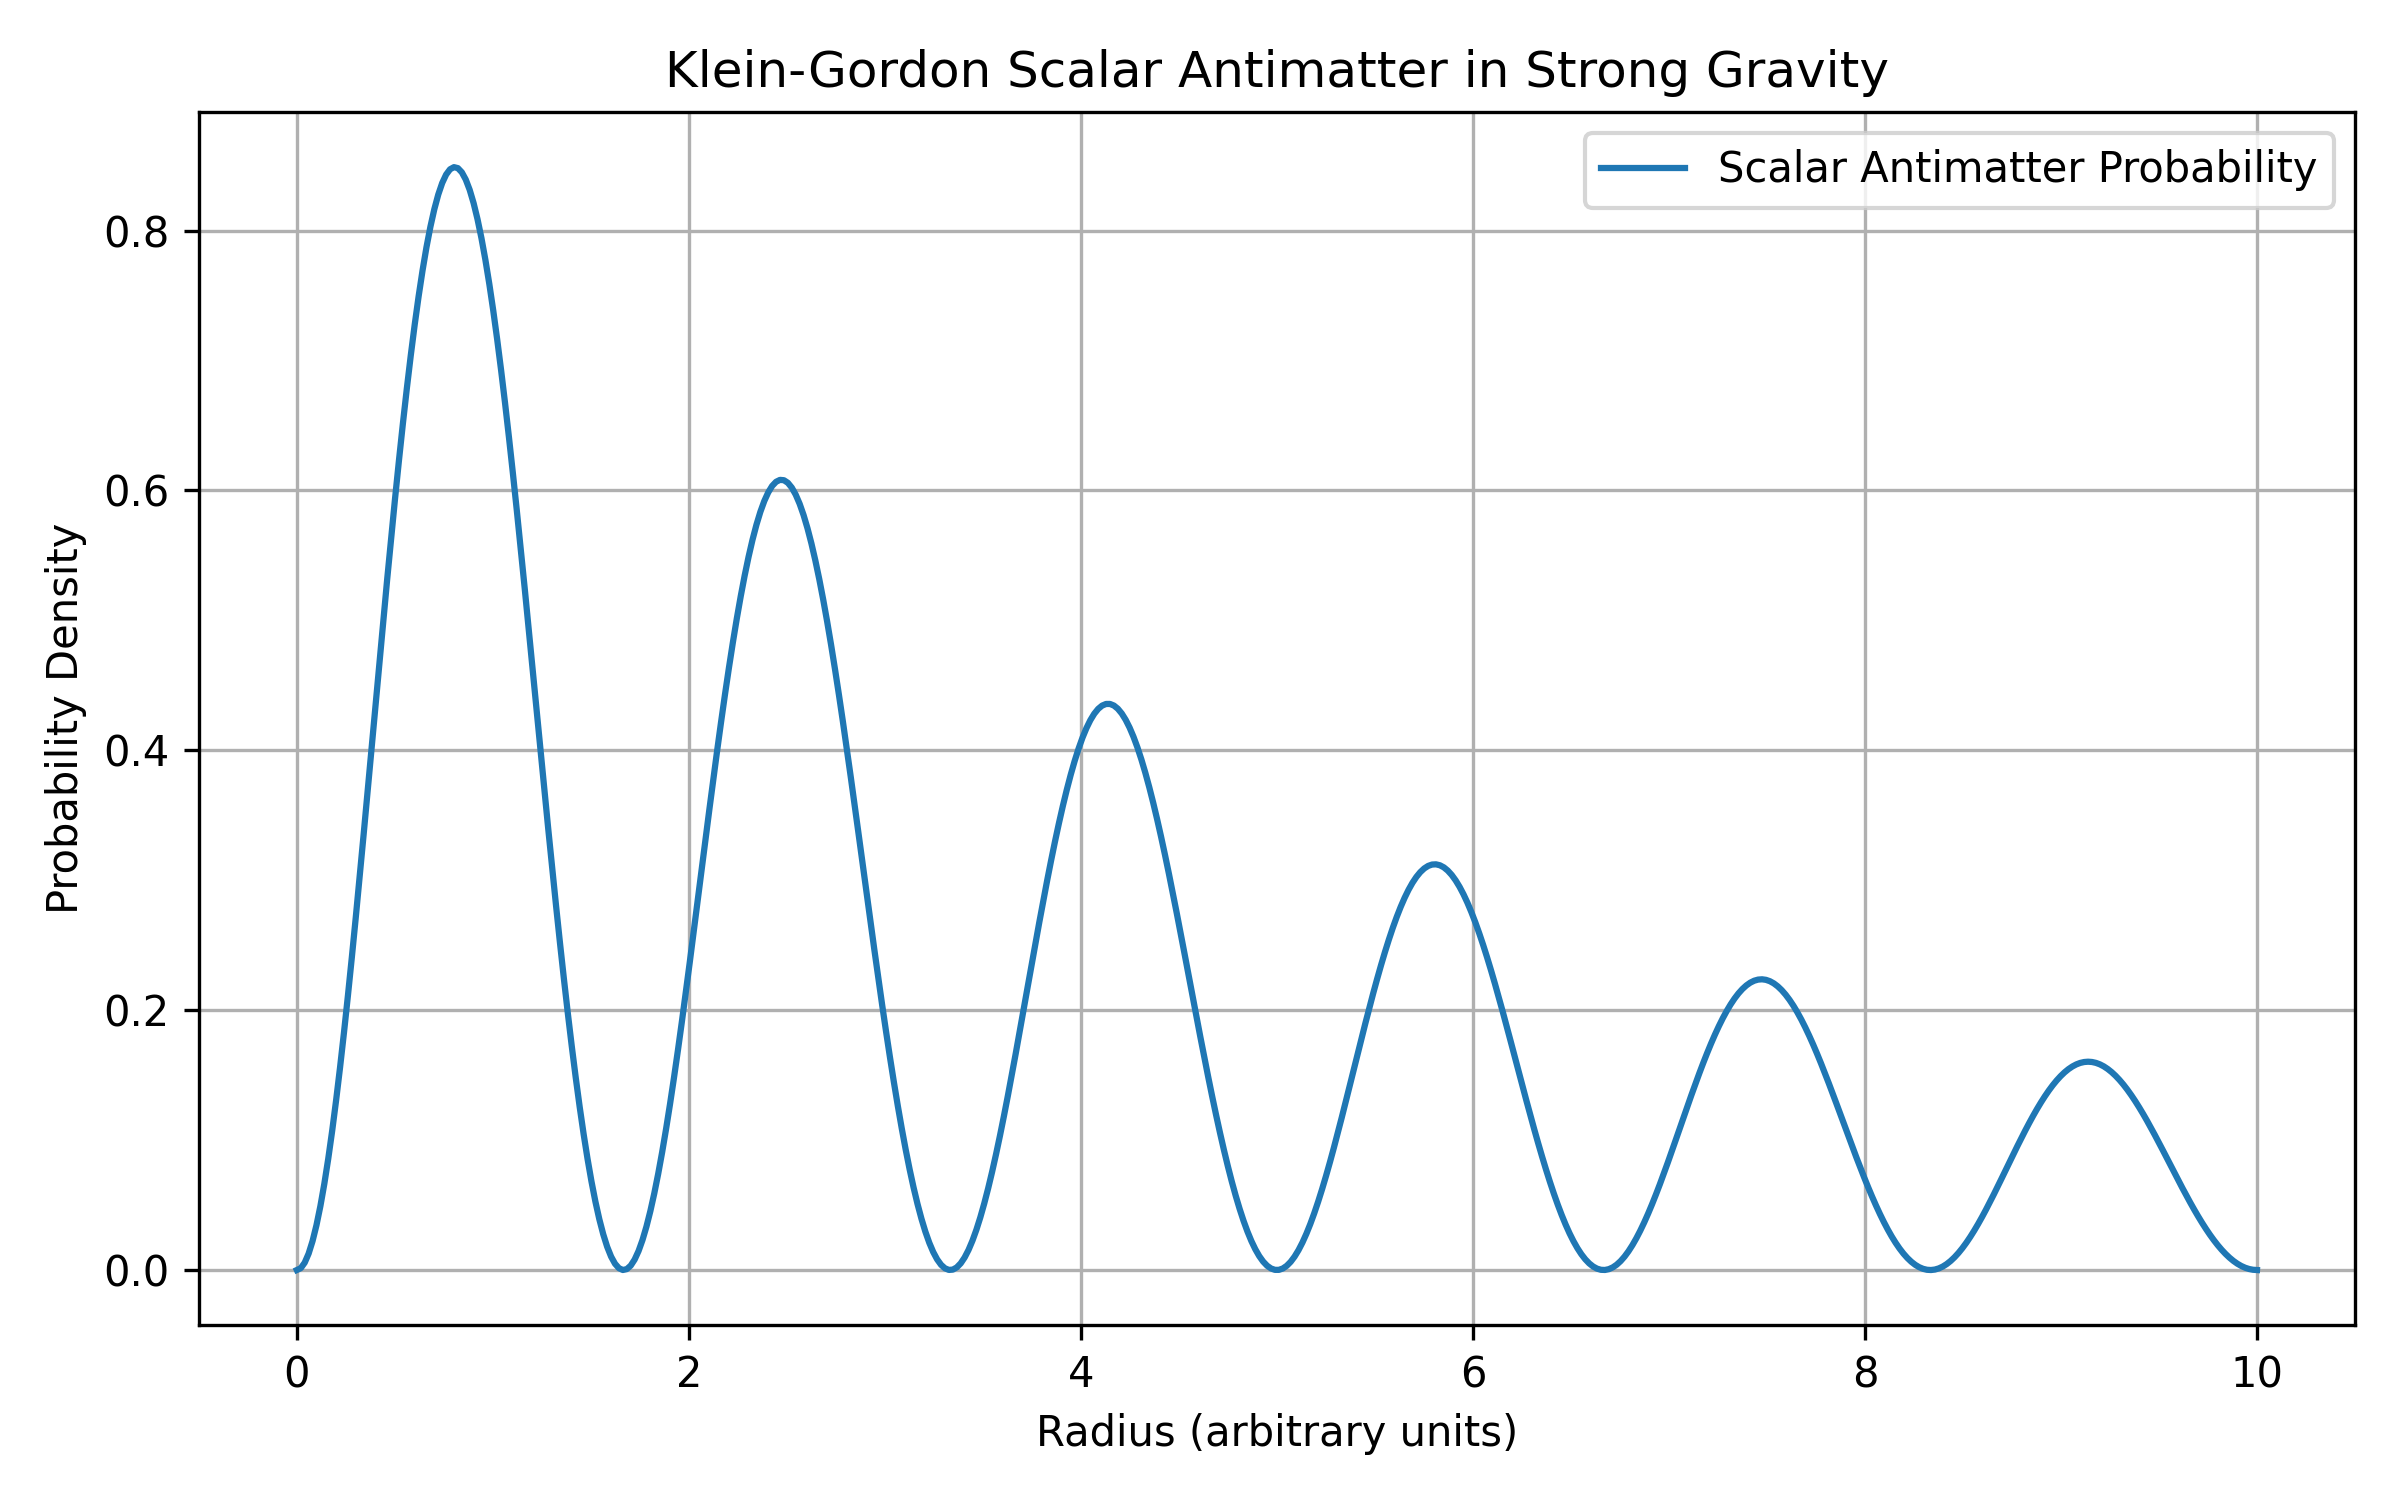
\includegraphics[width=0.8\textwidth]{kg_curved.png}
\caption{Probability distribution of scalar antimatter in strong gravity (placeholder).}
\label{fig:kg}
\end{figure}

\begin{figure}[H]
\centering
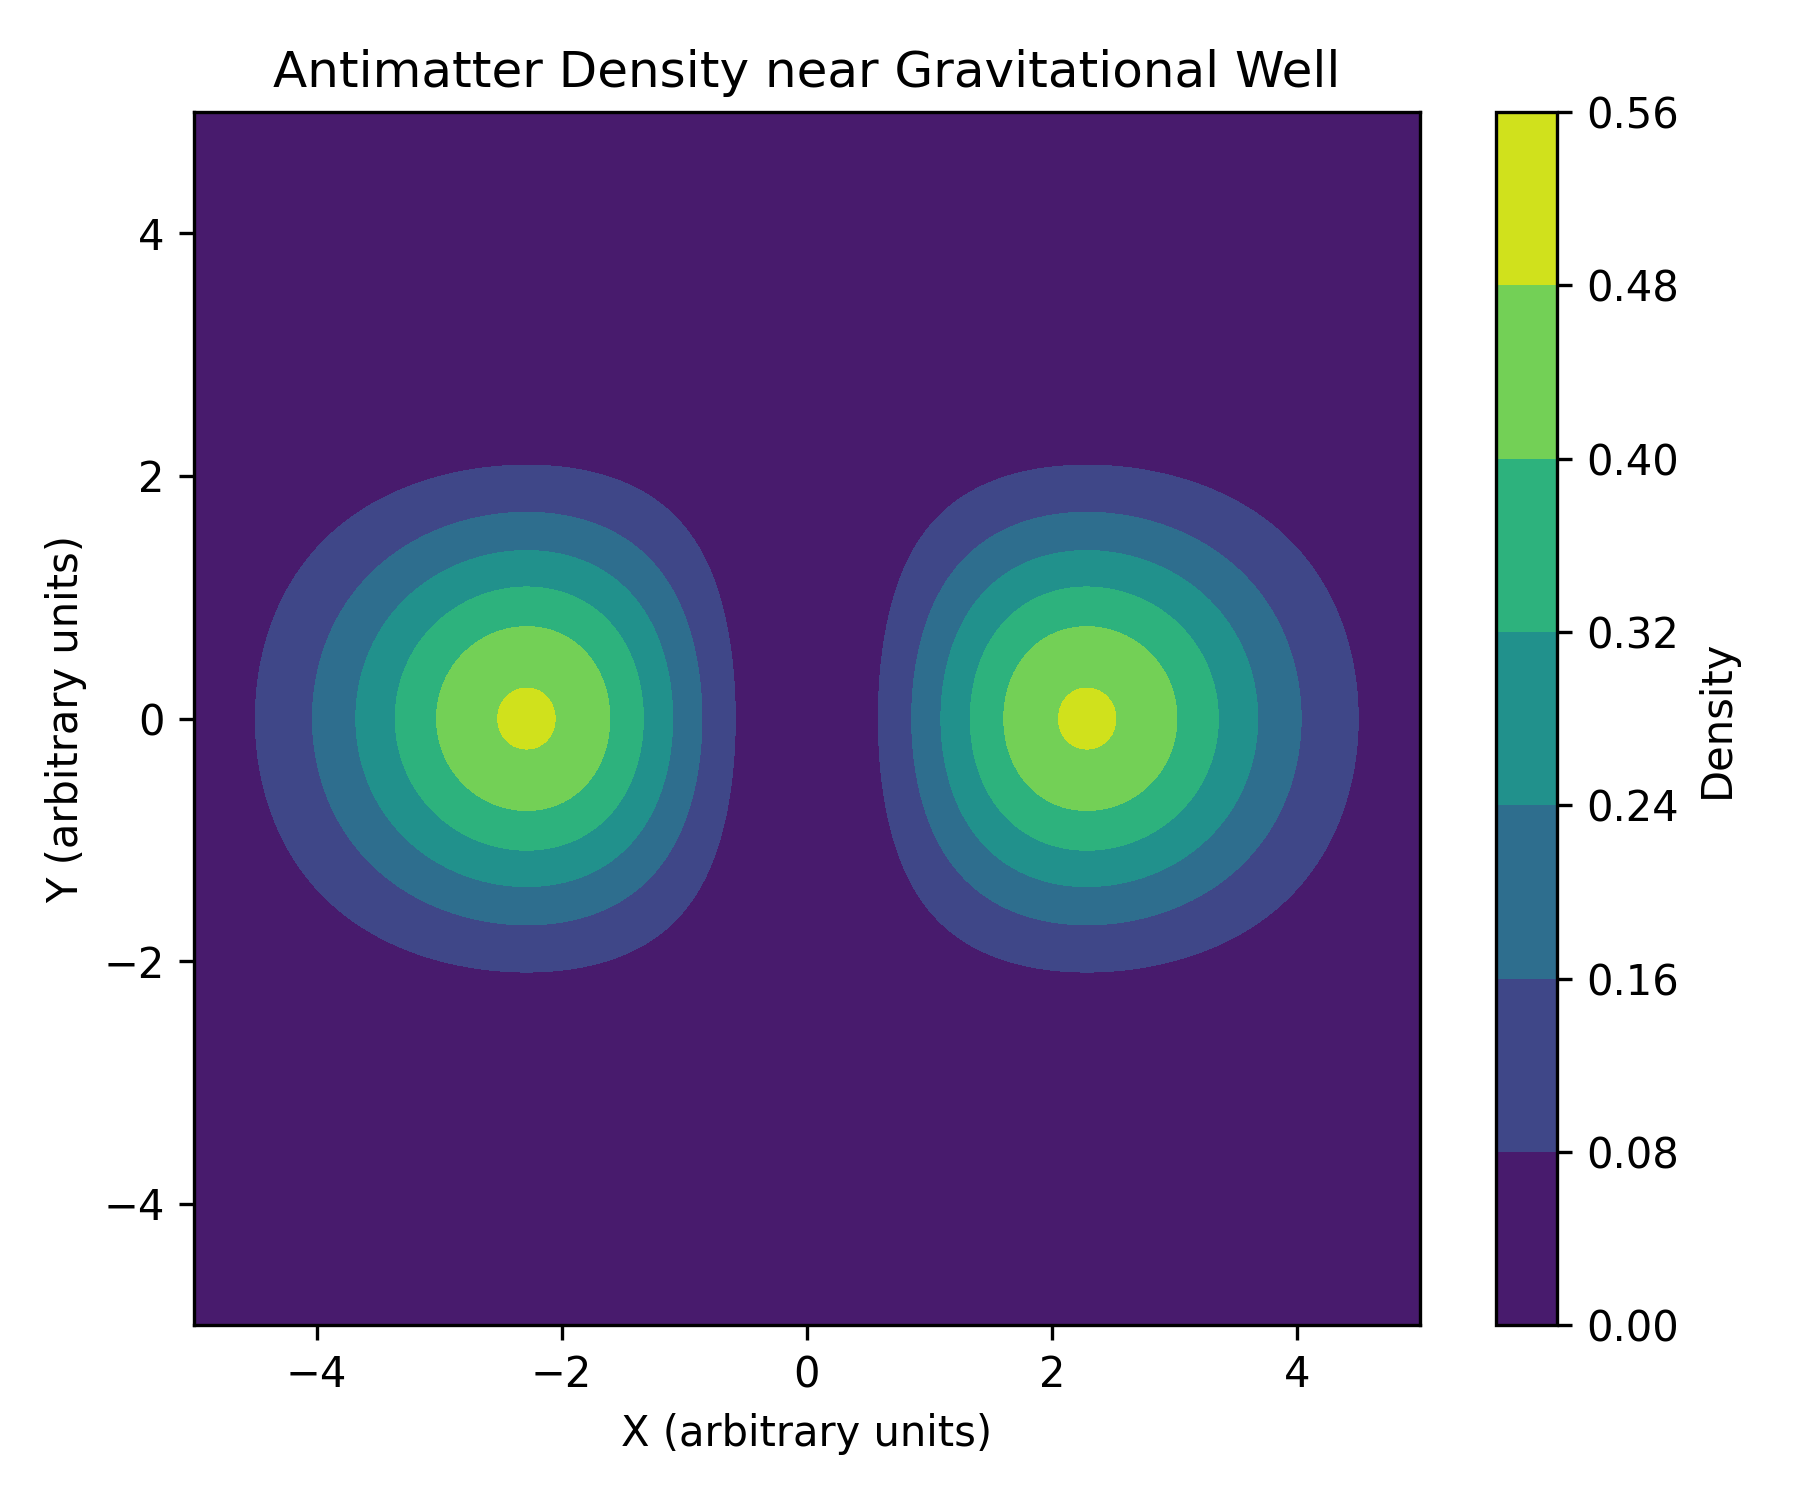
\includegraphics[width=0.8\textwidth]{antimatter_density.png}
\caption{Density map of antimatter near a gravitational well (example numerical result).}
\label{fig:dens}
\end{figure}

\section{Discussion }
The framework presented provides a clear and executable sequence from field equations to Hamiltonian construction and numerical solutions using spectral methods. Key points:
\begin{itemize}
  \item \textbf{Bound states:} Existence of square-integrable \(\chi(\mathbf{x})\) indicates localized antimatter confinement and potential distinctive annihilation signatures.
  \item \textbf{Metric sensitivity:} Geometrical parameters affect energy spectra and stability of states.
  \item \textbf{Interactions:} Electromagnetic fields and multi-particle effects significantly modify distributions and annihilation rates.
  \item \textbf{Limitations:} Approaching full QFT effects in curved spacetime requires advanced frameworks beyond PDE solutions.
\end{itemize}

\section{Conclusion }
In this work, we presented a comprehensive and interconnected framework for modeling the dynamics of antimatter in strong gravitational fields. By starting from the fundamental curved-space Dirac and Klein-Gordon equations, constructing the Hamiltonian in a 3+1 split, and applying both perturbative and spectral numerical methods, we provided a full pipeline from theoretical formulation to practical observables.

Key outcomes and insights include:
\begin{itemize}
    \item \textbf{Unified theoretical approach:} The sequence from field equations to Hamiltonian and perturbative expansions ensures that all derived quantities are consistently connected to the underlying physics.
    \item \textbf{Predictive power:} Computation of probability densities, currents, Wigner functions, and annihilation rates provides a quantitative basis to anticipate how antimatter behaves near high-curvature regions, such as neutron stars or black holes.
    \item \textbf{Sensitivity to geometry:} The methodology highlights the dependence of bound states and energy spectra on metric parameters, enabling parametric studies and scenario simulations.
    \item \textbf{Numerical applicability:} Spectral decomposition and truncated basis methods are feasible and flexible for a wide range of gravitational scenarios, offering convergence and control over numerical precision.
    \item \textbf{Limitations and future directions:} While our approach captures first-order quantum effects in curved spacetime, phenomena such as particle creation, back-reaction, and strong-field QFT effects require more advanced frameworks. Future work could integrate these aspects, alongside more complex interactions and electromagnetic fields, to extend predictive accuracy.
\end{itemize}

Overall, this framework establishes a solid foundation for both theoretical and numerical investigations of antimatter in extreme gravitational environments. The next steps include implementing full-scale simulations for specific astrophysical metrics, analyzing sensitivity to various parameters, and exploring potential observational signatures in high-energy astrophysics contexts.

\end{document}